\chapter{System}
The purpose of this chapter is to introduce the System in more details, Overall we are using for this work a Python script. The library  used in this work are: Request,JSON,Os,Subprocess,Getpass,Sys,Urllib3.
The use of the The Request library was for creating the interaction with the Web services of XNAT. The Python Requests library is the go-to solution for making HTTP requests in Python, thanks to its elegant and intuitive API that simplifies the process of interacting with web services and consuming data in the application.\footnote{https://www.datacamp.com/tutorial/python-subprocess} The sys module in Python provides access to variables and functions that interact closely with the Python interpreter and runtime environment. 

The fact that a JSON command is written the use of the JSON library was necessary. JSON is a syntax for storing and exchanging data.it a text, written with JavaScript object notation.\footnote{schoolW3, Phython JSON}
The Python subprocess module is a tool that allows to run other programs or commands from your Python code. Using the Python subprocess module is like giving commands to your computer using Python instead of typing them directly into the command prompt. This module makes it easy to automate the Python code.\footnote{https://www.datacamp.com/tutorial/python-subprocess}. Getpass() prompts the user for a password without echoing. The getpass module provides a secure way to handle the password prompts where programs interact with the users via the terminal.\footnote{https://www.geeksforgeeks.org/python/getpass-and-getuser-in-python-password-without-echo/}
 The import of urllib3 was to disable the InsecureRequestWarning, which is normally shown when requests connects to a site with an unverified SSL certificate. This approach helps keep the output clean and free of unnecessary warnings during the run of the Script.
 Currently the System is running Docker Engine 28.3.0,The Docker Client version in use is 20.10.5+dfsg1, which communicates with the Docker Engine to issue commands and manage images and containers. The XNAT web application is running on version 1.9.1.1, as verified through the web interface. 
 

\begin{figure}
    \centering
    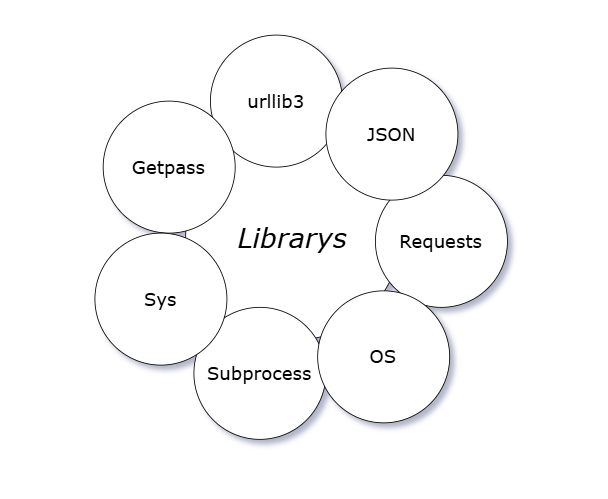
\includegraphics[width=0.7\linewidth]{en/content/lp.png}
    \caption{Schema: Core Libraries for Python Scripting in System Integration }
    \label{fig:enter-label}
\end{figure}


\section{Architecture and organization of the Code:}
 The automation script is structured into 17 distinct parts, each responsible for a specific step in the overall workflow.
 During the development of the automation script, i closely followed the steps of the manual process, since I had already tested and completed it manually. I carefully repeated the same steps during the implementation. In other words in every structured part is composed from a function that is responsible of doing a step of the manual Process.
 
 \section{The Dockerfile:}
 
The first function is responsible for writing the dockerfile, the function is called \texttt{def write\_dockerfile} and it takes three arguments the target directory for the dockerfile, the name of the Python script to include, and an optional base Docker image (defaulting to python:3.10-slim, currently the fastest and the slimest image of docker). The function creates the necessary folder (if it doesn't already exist), constructs the Dockerfile content, and writes it. The content of the dockerfile is introduced with a string interpolation and it containts the base image and numerous commands like WORKDIR /app (A working directory ) \texttt{COPY \{script\_filename\} /app/\{script\_filename\}} to copy the user skript inside of the image. The line  RUN pip install \texttt{--no-cache-dir pandas} tells Docker to install the pandas Python library using pip during the build process of the Docker image.  which helps reduce the overall image size and avoids unnecessary layers in the building process. The last component of the dockerfile is the \texttt{COPY requirements.txt /app/requirements.txt}, in this part it gives the opportunity for the user to write in a separate text file all the libraries used in the container script, which can be used later in the image build process.
i removed the CMD instruction from the Dockerfile because it caused errors when running the container in XNAT. The issue was due to a conflict between the CMD instruction in the Dockerfile and the command.json configuration, as both included the python3 prefix. This led to a duplicate command execution, which caused the container to fail. By removing CMD in the Dockerfile, the execution logic is now fully controlled by XNAT through the command.json, ensuring proper behavior during container launch.

\begin{lstlisting}[language=bash]
FROM python:3.10-slim
WORKDIR /app
COPY script.py /app/script.py
RUN pip install --no-cache-dir pandas
COPY requirements.txt /app/requirements.txt
\end{lstlisting}
The rest of the \texttt{def write\_dockerfile} ensures that the specified directory exists, then creates and writes a Dockerfile to that location.It constructs the full path to the file, writes the generated content into it, prints a confirmation message.


\lstset{
  language=Python,
  basicstyle=\ttfamily\small\color{black},
  keywordstyle=\color{black},
  identifierstyle=\color{black},
  stringstyle=\color{black},
  commentstyle=\color{black},
  numberstyle=\color{black},
  showstringspaces=false
}

\begin{lstlisting}
os.makedirs(docker_dir, exist_ok=True)
dockerfile_path = os.path.join(docker_dir, "Dockerfile")
with open(dockerfile_path, "w") as f:
    f.write(dockerfile_content)
print(f"Dockerfile written to {dockerfile_path}")
return dockerfile_path
\end{lstlisting}

This function ensure that the dockerfile will be written in a appropriate way and it secures that all the dependencies are stored in the external requirement text file. It handles all possible cases and avoid the issues of errors and the Stdin errors. 

\section{Building, Pushing and Tagging the image :}

when a command is deployed in XNAT and a container is being launched, the first thing that XNAT is controlling if the docker image is available in the DockerHub. Which means the user has to have essentially a account in the Docker hub, and preferably to log himself before using the following script.  consequently its essential to push and tag the image created.
The function responsible for the build is the \texttt{def build\_docker\_image}. and its expecting two parameters: 
\texttt{dockerfile\_path } for the Dockerfile path and the the name/tag for the Docker image to be built \texttt{docker\_image\_name}. For the build we used subprocess.run to call the external docker build command.
usually when we want to build an image in docker we use the basic command \texttt{docker built  .} 


\begin{lstlisting}
 build_result = subprocess.run(["docker", "build", "-f", dockerfile_path, "-t", docker_image_name, "."],  capture_output=True, text=True)
    if build_result.returncode != 0:
        print(f"Build failed:\n{build_result.stderr}")
        sys.exit(1)
\end{lstlisting}

As we can see in this block it showing  subprocess.run was used  to call the external docker build command and the -f ,dockerfile\_path, tells Docker which Dockerfile to use.The  -t ,docker\_image\_name, sets the name and tag for the image. The point (.) at the end of the command means the current directory will be used as the build context. In addition the \texttt{capture\_output=True} collects both stdout and stderr so the script can handle their output or errors, and the text=True makes sure outputs are returned as strings.
\\Now that the image has been succesfully built we can proceed  to the next essential Step:  "pushing the image to Docker Hub". In order to do that the same method by building of \texttt{subprocess.run} is used.


\begin{lstlisting}
full_tag = f"{dockerhub_username}/{docker_image_name}"
print(f"Pushing image to Docker Hub as '{full_tag}'...")
    push_result = subprocess.run(["docker", "push", full_tag], capture_output=True, text=True)
    if push_result.returncode != 0:
        print(f"Push failed:\n{push_result.stderr}")
        sys.exit(1)

\end{lstlisting}

In normal cases we use the comamnd \texttt{docker push the imagename}, and this assumes that the user is already logged in to their Docker account. However, in the automation script we make use of the \texttt{subprocess.run}. 
To explain this block,we begin by discussing the reason for using the full tag image. It constructs a full image tag in the Docker Hub format. Since the Docker Hub need image tags  to be in the format: The full image tag follows the format \texttt{dockerhub\_username/image\_name[:tag]}.

This line creates a correctly formatted name for your Docker image, so it links your Docker Hub account \texttt{(dockerhub\_username)} with the chosen image and optional version tag \texttt{(docker\_image\_name)}.

The line of the code: 
\begin{lstlisting}
push_result = subprocess.run(["docker", "push", full_tag], capture_output=True, text=True)
\end{lstlisting}
refers to the push process with the \texttt{subprocess.run} methode. And it follows the same concept as builing the Docker image. 

\section{The Prompt Function for the required input:}

 This function performs the task of capturing input from the user.
 We have used this function in the script in multiple scenarios. First of them to take the Docker Hub user name from the user, in order to customize the JSON command we asked the user about the name of the Command and her description, And overall, it is used to take the username and password from the user's login credentials.The function proceeds through all of this steps by running the script.
 The function looks like this:\\
 \begin{lstlisting}
 def get_input(prompt):
    while True:
        value = input(prompt)
        if value.strip():
            return value
        else:
            print("Cannot be empty.")

\end{lstlisting}
The \texttt{ def get\_input} uses a while True loop to keep asking until the user enters a input, the \texttt{value.strip()} removes any whitespace from the user input.If the input is valid the value is returned, if it not the \texttt{Cannot be empty} will be printed.


\section{The JSON Command :}





Demain 6 Rubliques dans le plan.

 
2. Architecture et Organisation du Code:
Structure:
Décrire la structure du code (modules, classes, fonctions) et son organisation en fichiers.
Modularité:
Expliquer comment le code est divisé en modules ou fonctions pour une meilleure lisibilité et maintenabilité.
API:
Si applicable, décrire l'interface de programmation (API) du code, en détaillant les entrées et sorties des fonctions principales. 
3. Algorithmes et Fonctionnalités:
Algorithmes:
Expliquer les algorithmes utilisés, leur complexité, et leurs fonctions spécifiques.
Fonctionnalités:
Décrire les principales fonctionnalités du code et leur rôle dans la recherche.
Interactions:
Expliquer comment le code interagit avec les données, que ce soit en entrée ou en sortie. 
'''